\documentclass[portuguese,aspectratio=169]{beamer}
\usetheme{Luebeck}
\usecolortheme{dove}
\usepackage{babel}
\usepackage{xcolor}

% Change standard block colors
% 1- Block title (background and text)
\setbeamercolor{block title}{bg=gray!30, fg=white}
% 2- Block body (background)
\setbeamercolor{block body}{bg=cyan!10}

%\setbeamerfont{description item}{series=\bfseries}
\setbeamercolor{description item}{fg=gray!70}

\title{Algebra Abstrata nas Telecomunicações}
\author{Leonardo Araújo}
\date{\today}

% https://sites.math.rutgers.edu/~sussmann/papers/z11.pdf
% https://meenalpathak.wordpress.com/2017/12/02/euclidean-algorithm-and-euclidean-decoder/
% https://www.youtube.com/watch?v=CcZf_7Fb4Us
% https://www.youtube.com/watch?v=1pQJkt7-R4Q
\begin{document}

\frame{\titlepage}

\begin{frame}
\frametitle{Introdução}
\begin{itemize}
    \item Uma breve introdução à Álgebra Abstrata\\
    \textcolor{gray}{Álgebra abstrata é um ramo da matemática que estuda estruturas algébricas tais como \textcolor[gray]{0.2}{grupos, anéis, e corpos}. 
    Estas estruturas fornecem a base para o entendimento e generalização de operações algébricas.}
    \item Importância na matemática e aplicações\\
    \textcolor{gray}{A álgebra abstrata é crucial em vários campos, fornecendo uma base teórica e ferramentas práticas para resolver problemas complexos em
    \textcolor[gray]{0.2}{criptografia, teoria da codificação e ciência da computação}.}
\end{itemize}
\end{frame}

\begin{frame}[allowframebreaks]
\frametitle{Grupos, anéis e corpos}
\textbf{Grupos}

Um grupo é um conjunto de elementos associados a uma operação.

\begin{block}{Definição}
  Seja $G$ um conjunto não vazio e $*$ uma operação binária definida sobre $G$. O par ordenado $(G,*)$ é um grupo se são satisfeitas os seguintes axiomas:
  \begin{description}
    \item[Fecho] $\forall *$, se $a,b \in G$ e dado $a * b = c$, então $c \in G$.
    \item[Associatividade] $\forall a,b,c \in G$ temos $(a * b) * c = a * (b * c)$.
    \item[Elemento neutro] $\exists e \in G \mid e*a=a*e=a$, $\forall a \in G$.
    \item[Elemento simétrico] $\forall a \in G$, $\exists a' \in G \mid a * a' = a' * a = e$, onde $e$ é o elemento neutro ($a'$ é o elemento inverso de $a$).
    \item[Comutatividade] (grupo abeliano) $\forall a, b \in G$, $a * b = b * a$.
  \end{description}
\end{block}

\framebreak
\begin{block}{Exemplos}
  \begin{itemize}
    \item O conjunto $G=\{0,1\}$ com a operação $\oplus$ (ou exclusivo, ou soma módulo 2) é um grupo.
    \item O conjunto dos inteiros sob adição $(\mathbb{Z},+)$ é um grupo.
    \item $(\mathbb{Z}_n,+)$ o conjunto dos inteiros entre $0$ e $n-1$ com soma módulo $n$ é um grupo.
  \end{itemize}
\end{block}

\framebreak
\textbf{Anel}

Anel é um conjunto equipado com duas operações binárias que satisfazem propriedades análogas às da adição e multiplicação em inteiros.

\textcolor{gray}{Formalmente, um anel é um conjunto dotado de duas operações binárias chamadas adição e multiplicação, de modo que o anel é um grupo abeliano em relação ao operador de adição, e o operador de multiplicação é associativo, é distributivo sobre a operação de adição e tem uma identidade multiplicativa. elemento.}

\framebreak
\begin{block}{Definição}
\fontsize{11pt}{12pt}\selectfont
Um anel $R$ é um conjunto equipado com duas operações binárias: $+$ (adição) e $\cdot$ (multiplicação) satisfazendo os seguintes axiomas:
  \begin{itemize}
    \item $R$ é um grupo abeliano sob adição, ou seja
      \begin{description}
        \item[$+$ é associativa] $(a + b) + c = a + (b + c)$, $\forall a,b,c \in R$ ($+$ é associativa),
        \item[$+$ é comutativa] $a + b = b + a$, $\forall a,b,c \in R$ ($+$ é comutativa),
        \item[$+$ possui elemento identidade] $\exists 0 \in R \mid a + 0 = a$,
        \item[$+$ possui inversa] para cada $a \in R, \exists -a \in R | a + (-a) = 0$;
      \end{description}
    \item $R$ é um monoide sob a multiplicação, ou seja,
      \begin{description}
        \item[Multiplicação é associativa] $(a \cdot b) \cdot c = a \cdot (b \cdot c)$, $\forall a,b,c \in R$,
        \item[Elemento identidade da multiplicação] $\exists 1 \in R \mid a \cdot 1 = a \text{ e } 1 \cdot a = a, \forall a \in R$;
      \end{description}
  \end{itemize}
  \begin{description}
    \item[Distributividade] a multiplicação é distributiva com relação à adição:
      \begin{itemize}
        \item $a \cdot (b + c) = (a \cdot b) + (a \cdot c), \forall a, b, c \in R$,
        \item $(b + c) \cdot a = (b \cdot a) + (c \cdot a), \forall a, b, c \in R$.
      \end{itemize}
  \end{description}
\end{block}

\framebreak
\begin{block}{Exemplos}
  \begin{itemize}
    \item Os inteiros com operações de adição e multiplicação.
    \item Os números racionais, reais e complexos são anéis comutativos do tipo corpo.
  \end{itemize}
\end{block}



\framebreak
\textbf{Corpo}

Corpo é um conjunto equipado com duas operações binárias adição, subtração, multiplicação e divisão que satisfazem propriedades análogas àquelas nos números racionais e reais.

\framebreak
\begin{block}{Definição}
Um corpo $F$ é um conjunto equipado com duas operações binárias: $+$ (adição) e $\cdot$ (multiplicação) satisfazendo os seguintes axiomas:
  \begin{description}
    \item[Associatividade] $a + (b + c) = (a + b) + c$ e $a \cdot (b \cdot c) = (a \cdot b) \cdot c$,
    \item[Comutatividade] $a + b = b + a$ e $a \cdot b = b \cdot a$,
    \item[Identidade] $\exists 0, 1 \in F$ distintos tais que $a + 0 = a$ e $a \cdot 1 = a$,
    \item[Inversa] $\exists -a, a^{-1} \in F$ distintos tais que $a + (-a) = 0$ e $a \cdot a^{-1} = 1$,
    \item[ou seja] ($F$ é um grupo abeliano sob adição com elemento neutro $0$ e também um grupo não-nulo abeliano sob a multiplicação com elemento neutro $1$)
    \item[Distributividade] da multiplicação sobre a adição $a \cdot (b + c) = (a \cdot b) + (a \cdot c)$.
  \end{description}
\end{block}

\framebreak
\begin{block}{Exemplos}
  \begin{itemize}
    \item Os inteiros com operações de adição e multiplicação.
    \item Os números racionais, reais e complexos.
    \item Muitos protocolos criptográficos utilizam corpos finitos (também chamados de corpos de Galois): RSA (Rivest-Shamir-Adleman), ECC (Elliptic Curve Cryptography), AES (Advanced Encryption Standard), Diffie-Hellman, etc.
    \item Código Reed-Solomon (detecção e correção de erros).
  \end{itemize}
\end{block}

\framebreak
\begin{block}{Corpo primo $GF(p)$ -- corpo finito (\emph{Galois field})}
  Seja $p$ um primo, o conjunto $\{0,1,\ldots,p-1\}$ é um corpo de ordem $p$ sob a
  adição e multiplicação módulo $p$.
\end{block}

Exemplo: $p=7$
\begin{table}[!htb]
    \begin{minipage}{.5\linewidth}
      \caption{Adicção módulo 7.}
      \centering
        \begin{tabular}{l|lllllll}
          $+$ & 0 & 1 & 2 & 3 & 4 & 5 & 6 \\
          \hline
          0 & 0 & 1 & 2 & 3 & 4 & 5 & 6 \\
          1 & 1 & 2 & 3 & 4 & 5 & 6 & 0 \\
          2 & 2 & 3 & 4 & 5 & 6 & 0 & 1 \\
          3 & 3 & 4 & 5 & 6 & 0 & 1 & 2 \\
          4 & 4 & 5 & 6 & 0 & 1 & 2 & 3 \\
          5 & 5 & 6 & 0 & 1 & 2 & 3 & 4 \\
          6 & 6 & 0 & 1 & 2 & 3 & 4 & 5
        \end{tabular}
    \end{minipage}%
    \begin{minipage}{.5\linewidth}
      \centering
        \caption{Multiplicação módulo 7.}
        \begin{tabular}{l|lllllll}
        $\cdot$ & 0 & 1 & 2 & 3 & 4 & 5 & 6 \\
        \hline
        0 & 0 & 0 & 0 & 0 & 0 & 0 & 0 \\
        1 & 0 & 1 & 2 & 3 & 4 & 5 & 6 \\
        2 & 0 & 2 & 4 & 6 & 1 & 3 & 5 \\
        3 & 0 & 3 & 6 & 2 & 5 & 1 & 4 \\
        4 & 0 & 4 & 1 & 5 & 2 & 6 & 3 \\
        5 & 0 & 5 & 3 & 1 & 6 & 4 & 2 \\
        6 & 0 & 6 & 5 & 4 & 3 & 2 & 1
        \end{tabular}
    \end{minipage} 
\end{table}

\end{frame}

\begin{frame}[allowframebreaks]
  \frametitle{Corpo Binário} 
  Os campos de Galois de ordem $2^p$ são amplamente utilizados na comunicação
  digital devido à sua compatibilidade com a lógica binária, a eficiência nas
  operações aritméticas e sua aplicação em códigos de detecção e correção de
  erros. Em sistemas digitais e computadores, que operam com lógica binária, os
  elementos desses campos podem ser representados naturalmente como vetores
  binários de comprimento $p$. As operações aritméticas nesses campos, como a
  adição e a multiplicação, podem ser implementadas de forma eficiente
  utilizando operações bit a bit, o que é crucial para o processamento em tempo
  real em sistemas de comunicação. Além disso, muitos códigos de correção de
  erros, como os códigos Reed-Solomon e BCH, são definidos sobre campos de
  Galois de ordem $2^p$, fornecendo propriedades robustas e algoritmos de
  decodificação eficientes. Essa compatibilidade com a estrutura binária dos
  sistemas digitais torna os campos de Galois de ordem $2^p$ ideais para
  garantir uma comunicação confiável e eficiente.


  \framebreak
  %Podemos ter um corpo finito $GF(q)$ com $q$ primo ou uma potência de $p$.

  Um polinômio $f(X)$ na variável $X$ com coeficientes em $GF(2)$ é da forma:
  \begin{equation}
    f(X) = f_0 + f_1 X + f_2 X^2 + \ldots + f_n X^n
  \end{equation}
  onde $f_i = 0 \text{ou} 1$, para $0 \leq i \leq n$.

  Existem $2^n$ polinômios em $GF(2)$ com grau $n$.
  \begin{block}{Exemplo}
  Para $n=2$: $X^2$, $1+X^2$, $X+X^2$ e $1+X+X^2$.
  \end{block}

  Dados dois polinômios $f(X)$ e $g(X)$ em $GF(2)$, de grau $n$ e $m$, respectivamente, com $m \leq n$,
  \begin{eqnarray}
    f(X) + g(X) =& (f_0 + g_0) + (f_1 + g_1) X + \ldots + (f_m + g_m) X^m + \nonumber\\
                  & + f_{m+1} X^{m+1} + \ldots + f_n X^n
  \end{eqnarray}
  \begin{block}{Exemplo}
    $f(X) = 1 + X^2 + X^3 + X^4 + X^7$ e $g(X) = 1 + X + X^3 + X^5$ 
    \begin{eqnarray}
      f(X) + g(X) &=& (1+1) + X + X^2 + (1+1) X^3 + X^4 + X^5 + X^7 \nonumber\\
                  &=& X + X^2 + X^4 + X^5 + X^7
    \end{eqnarray}
  \end{block}

  \framebreak
  A multiplicação de $f(X)$ e $g(X)$ é dada por
  \begin{equation}
    f(X) \cdot g(X) = c_0 + c_1 X + c_2 X^2 + \ldots + c_{n+m} X^{n+m}
  \end{equation}
  onde
  \begin{eqnarray}
    c_0 &=& f_0 g_0 \nonumber\\
    c_1 &=& f_0 g_1 + f_1 g_0 \nonumber\\
    c_2 &=& f_0 g_2 + f_1 g_1 + f_2 g_0 \nonumber\\
        &\vdots& \nonumber\\
    c_i &=& f_0 g_i + g_1 g_{i-1} + f_2 g_{i-2} + \ldots + f_i g_0 \nonumber\\
        &\vdots& \nonumber\\
    c_{n+m} &=& f_n g_m
  \end{eqnarray}

  \framebreak
  \begin{block}{Propriedades}
    Os polinômios em $GF(2)$ satisfazem as seguintes propriedades:
    \begin{description}
      \item[Comutatividade] $a(x) + b(X) = b(X) + a(X)$ e $a(x) \cdot b(X) = b(X) \cdot a(X)$
      \item[Associatividade] $a(X) + [b(X) + c(X)] = [a(X) + b(X)] + c(X)$ e $a(X) \cdot [b(X) \cdot c(X)] = [a(X) \cdot b(X)] \cdot c(X)$
      \item[Distributividade] $a(X) \cdot [b(X) + c(X)] = [a(X) \cdot b(X)] + [a(X) \cdot c(X)]$
    \end{description}
  \end{block}

  \framebreak
  Suponha $g(X)$ de grau não-nulo. Quando $f(X)$ é dividido por $g(X)$, obtemos um par único em $GF(2)$ de $q(X)$ (quociente) e $r(X)$ (resto) tal que
  \begin{equation}
    f(X) = q(X) g(X) + r(X)
  \end{equation}
  e o grau de $r(X)$ é menor do que o de $g(X)$.

  \framebreak
  \begin{block}{Exemplo}
    $f(X) = 1 + X + X^4 + X^5 + X^6$ e $g(X) = 1 + X + X^3$
    \[
      \begin{array}{rrrrrrrl}
        X^6 &+ X^5 &+ X^4 &&&+ X &+ 1 & \multicolumn{1}{| l}{X^3 + X + 1} \\
        \cline{8-8}
        \rule{0pt}{2.6ex}
        X^6 &&+ X^4 &+ X^3 &&& & X^3 + X^2 \\
        \cline{1-7}
        \rule{0pt}{2.6ex}
         & X^5 &&+ X^3 &&+ X &+ 1 & \\
         & X^5 &&+ X^3 &+ X^2 &&& \\
        \cline{2-7}
        \rule{0pt}{2.6ex}
         &&&& X^2 &+ X &+ 1 &
      \end{array}
    \]
    $q(X) = X^3 + X^2$ e $r(X) = X^2 + X + 1$
  \end{block}

  \framebreak
  Um polinômino de grau $n$ é irredutível se ele não é divisível por um polinômino de grau menor do que $n$.

  \begin{block}{Exemplo}
    $X^2$, $X^2+1$ e $X^2 + X$ são polinômios de grau 2 não irredutíveis pois são divisíveis por $X$ ou $X+1$.

    \vspace{2ex}
    $X^2 + X + 1$ não é divisível por $X$ nem $X+1$, sendo portanto um polinômino de grau 2 irredutível.

    \vspace{2ex}
    $X^3 + X + 1$ é um polinômio de grau 3 irredutível. $X^4 + X + 1$ é um polinômio de grau 4 irredutível.

    \vspace{2ex}
    Para $n \geq 1$ existe um polinômio irredutível de grau $n$.
  \end{block}

  \framebreak
  \begin{block}{Teorema}
    Um polinômio irredutível em $GF(2)$ de grau $n$ divide $X^{2^n-1}+1$.
  \end{block}

  \begin{block}{Exemplo}
    $m=3$\\
    $X^3+X+1$ divide $X^7+1$

    $X^7+1 = (X^3+X+1)(X^4 + X^2 + X + 1) + 0$
  \end{block}

  \framebreak
  Dizemos que um polinômio irredutível $p(X)$ de grau $m$ é primitivo se o menor inteiro positivo $n$ para o qual $p(X)$ divide $X^n+1$ é $n=2^m-1$.
  \begin{block}{Exemplo}
  Para $m=4$, $p(X)=X^4+X+1$ divide $X^{15}+1$ mas não divide $X^n+1$ para $1 \leq n < 15$. Desta forma, $X^4+X+1$ é um polinômio primitivo de grau 4.
  \end{block}

  \framebreak
  \begin{table}[h!]
    \centering
    \caption{Alguns polinômios primitivos em $GF(2)$ para grau $m$ de 3 a 24. Para alguns $m$ existem mais de um polinômio primitivo. Uma lista completa até $m=32$ pode ser vista \href{https://www.partow.net/programming/polynomials/primitive_polynomials_GF2.txt}{aqui}.}
    \begin{tabular}{llll}
        \hline
        grau (m) & polinômio primitivo & grau (m) & polinômio primitivo \\
        \hline
        \rule{0pt}{2.6ex}%
        3 & $X^3 + X + 1$ & 14 & $X^{14} + X^{10} + X^6 + X + 1$ \\
        4 & $X^4 + X + 1$ & 15 & $X^{15} + X + 1$ \\
        5 & $X^5 + X^2 + 1$ & 16 & $X^{16} + X^{12} + X^3 + X + 1$ \\
        6 & $X^6 + X + 1$ & 17 & $X^{17} + X^3 + 1$ \\
        7 & $X^7 + X^3 + 1$ & 18 & $X^{18} + X^7 + 1$ \\
        8 & $X^8 + X^4 + X^3 + X^2 + 1$ & 19 & $X^{19} + X^5 + X^2 + X + 1$ \\
        9 & $X^9 + X^4 + 1$ & 20 & $X^{20} + X^3 + 1$ \\
        10 & $X^{10} + X^3 + 1$ & 21 & $X^{21} + X^2 + 1$ \\
        11 & $X^{11} + X^2 + 1$ & 22 & $X^{22} + X + 1$ \\
        12 & $X^{12} + X^6 + X^4 + X + 1$ & 23 & $X^{23} + X^5 + 1$ \\
        13 & $X^{13} + X^4 + X^3 + X + 1$ & 24 & $X^{24} + X^7 + X^2 + X + 1$ \\
        \hline
    \end{tabular}
  \end{table}

  \framebreak
  Uma outra propriedade útil dos polinômios em $GF(2)$ é
  \begin{equation}
    [f(X)]^{2^i} = f(X^{2^i}).
  \end{equation}

   Demonstração:
   \begin{eqnarray}
     f^2(X) &=& (f_0 + f_1 X + \ldots + f_n X^n)^2 \nonumber\\
            &=& [f_0 + (f_1 X + f_2 X^2 + \ldots + f_n X^n)]^2 \nonumber\\
            &=& f^2_0 + f_0 \cdot (f_1 X + f_2 X^2 + \ldots + f_n X^n) \nonumber\\
             && + f_0 \cdot (f_1 X + f_2 X^2 + \ldots + f_n X^n) + (f_1 X + f_2 X^2 + \ldots + f_n X^n)^2 \nonumber\\
            &=& f^2_0 + (f_1 X + f_2 X^2 + \ldots + f_n X^n)^2 \nonumber\\
            &=& \vdots \nonumber\\
            &=& f^2_0 + (f_1 X)^2 + (f_2 X^2)^2 + \ldots (f_n X^n)^2 \nonumber\\
            &=& f^2_0 + f_1 X^2 + f_2 (X^2)^2 + \ldots f_n (X_n)^2 \nonumber \\
            &=& f(X^2)
   \end{eqnarray}
   onde utilizamos que $f^2_i = f_i$ uma vez que $f_i = 0\text{ ou }1$.

\end{frame}


\begin{frame}[allowframebreaks]
  \frametitle{Corpo Finito $GF(2^m)$}
  Os campos de Galois $GF(2^m)$ são estruturas algébricas extremamente importantes em diversas áreas da matemática aplicada, especialmente em teoria da informação, criptografia e comunicação digital.
  Seguem alguns exemplos de utilização:
  \begin{description}
    \item[Códigos de Correção de Erro]\hfill \\
      \begin{itemize}
        \item Códigos de Reed-Solomon -- utilizado em CDs, DVDs, códigos QR e transmissão de dados
        \item Códigos BCH -- comunicação via satélite, comunicação móvel, disco rígidos
        \item Códigos LDPC (\emph{Low-Density Parity-Check}) -- Wi-Fi, DVB-S2, redes 5G
      \end{itemize}
    \framebreak
    \item[criptografia]\hfill \\
      \begin{itemize}
        \item AES (\emph{Advanced Encryption Standard}) -- utiliza $GF(2^8)$ na construção dos \emph{S-box}
        \item Criptografia de Curva Elíptica (ECC, \emph{Elliptic Curve Cryptography}) -- definida em $GF(2^m)$
      \end{itemize}
    \item[processamento de sinais]\hfill \\
      \begin{itemize}
        \item FFT em corpos finitos -- utilizada para realizar de forma rápida convoluções e multiplicações polinomiais
        \end{itemize}
  \end{description}

  \framebreak
  $GF(2^m)$ pode ser construído a partir de um polinômio irredutível de grau $m$ sobre $GF(2)$.

  \vspace{2ex}
  Os elementos de $GF(2^m)$ podem ser representados como polinômios de grau menor que $m$ com coeficientes em ${0,1}$.

  \vspace{2ex}
  O polinômio irredutível é fundamental para a construção de $GF(2^m)$ porque
  ele define as regras de redução que garantem que todas as operações no campo
  resultem em elementos dentro do campo. Usando o polinômio irredutível,
  podemos gerar todos os elementos do campo e definir as operações de adição e
  multiplicação de forma consistente e eficiente.
\end{frame}

\begin{frame}[allowframebreaks]
  \frametitle{Construção de $GF(2^3)$}
  \begin{itemize}
  \item $m=3$
  \item Polinômio irredutível $p(X)=X^3+X^2+1$.
  \item $\alpha$ é um elemento primitivo, então $p(\alpha) = 0$, logo $\alpha^3 + \alpha^2 + 1 = 0$. Temos então $\alpha^3 = \alpha^2 + 1$.
  \item Os elementos em $F^\ast = \{0, 1, \alpha, \alpha^2, \ldots, \alpha^{2^m-2}\}$.
  \item $\alpha^4 = \alpha^3 \cdot \alpha = (\alpha^2 + 1) \cdot \alpha = \alpha^3 + \alpha = \alpha^2 + \alpha + 1$
  \item $\alpha^5 = \alpha^4 \cdot \alpha = (\alpha^2 + \alpha + 1) \cdot \alpha = \alpha^3 + \alpha^2 + \alpha = \alpha^2 + 1 + \alpha^2 + \alpha = \alpha + 1$
  \item $\alpha^6 = \alpha^5 \cdot \alpha = (\alpha + 1) \cdot \alpha = \alpha^2 + \alpha$
  \item Note que $\alpha^7 = 1$, $\alpha^8 = \alpha$, etc (cíclico, o conjunto $F^\ast$ possui apenas $2^{m}$ elementos distintos).
  \end{itemize}

  \framebreak
  \begin{table}
    \caption{Representação dos elementos de $GF(2^3)$ gerados por $p(X)=1+X^2+X^3$.}
    \begin{tabular}{lrrrl}
      potência & \multicolumn{3}{c}{polinômio} & 3-upla \\
      \hline
      0          & 0 & & & (0 0 0)\\ 
      1          & 1 & & & (1 0 0) \\
      $\alpha$   & & $\alpha$ & & (0 1 0) \\
      $\alpha^2$ & & & $\alpha^2$ & (0 0 1) \\
      $\alpha^3$ & 1 & & $+\alpha^2$ & (1 0 1) \\
      $\alpha^4$ & 1 & $+\alpha$ & $+\alpha^2$ & (1 1 1) \\
      $\alpha^5$ & 1 & $+\alpha$ & & (1 1 0) \\
      $\alpha^6$ & & $\alpha$ & $+\alpha^2$ & (0 1 1)
    \end{tabular}
  \end{table}
\end{frame}

\begin{frame}
  \frametitle{Construção de $GF(2^4)$}
  \begin{footnotesize}
  \begin{table}
    \caption{Representação dos elementos de $GF(2^4)$ gerados por $p(X)=1+X+X^4$.}
    \begin{tabular}{lrrrrl}
      potência & \multicolumn{4}{c}{polinômio} & 4-upla \\
      \hline
      0          & 0 & & & & (0 0 0 0)\\ 
      1          & 1 & & & & (1 0 0 0) \\
      $\alpha$   & & $\alpha$ & & & (0 1 0 0) \\
      $\alpha^2$ & & & $\alpha^2$ & & (0 0 1 0) \\
      $\alpha^3$ & & & & $\alpha^3$ & (0 0 0 1) \\
      $\alpha^4$ & 1 & $+\alpha$ & & & (1 1 0 0) \\
      $\alpha^5$ & & $\alpha$ & $+\alpha^2$ & & (0 1 1 0) \\
      $\alpha^6$ & & & $\alpha^2$ & $+\alpha^3$ & (0 0 1 1)\\
      $\alpha^7$ & 1 & $+\alpha$ & & $+\alpha^3$ & (1 1 0 1) \\
      $\alpha^8$ & 1 & & $+\alpha^2$ & & (1 0 1 0) \\
      $\alpha^9$ & & $\alpha$ & & $+\alpha^3$ & (0 1 0 1) \\
      $\alpha^{10}$ & 1 & $\alpha$ & $+\alpha^2$ & & (1 1 1 0) \\
      $\alpha^{11}$ & & $\alpha$ & $+\alpha^2$ & $+\alpha^3$ & (0 1 1 1) \\
      $\alpha^{12}$ & 1 & $+\alpha$ & $+\alpha^2$ & $+\alpha^3$ & (1 1 1 1) \\
      $\alpha^{13}$ & 1 & & $+\alpha^2$ & $+\alpha^3$ & (1 0 1 1) \\
      $\alpha^{14}$ & 1 & & & $+\alpha^3$ & (1 0 0 1)
    \end{tabular}
  \end{table}
  \end{footnotesize}
\end{frame}

\begin{frame}[allowframebreaks]
\frametitle{Aritmética modular}

\begin{figure}
  \centering
  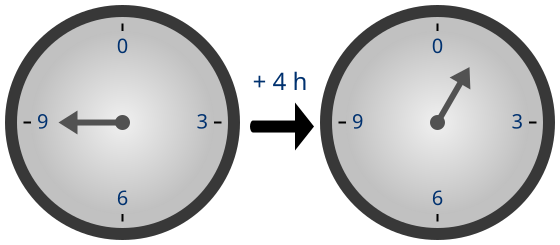
\includegraphics[width=0.5\textwidth]{clock_group.png}
  \caption{Relógio: exemplo de aritmética módulo 12}\label{fig-clockgroup}
\end{figure}

\begin{block}{Definição}
Dado um inteiro $m \geq 1$, chamado módulo, dois inteiros $a$ e $b$ são congruentes módulo $m$, se $m$ é um divisor da diferença entre eles ($a-b \mid m$), ou seja,
se existe um inteiro $k$ tal que
\begin{equation}
  a - b = k m.
\end{equation}
Denotamos a congruência entre $a$ e $b$ através da expressão
\begin{equation}
  a \equiv b \mod m
\end{equation}
\end{block}

\begin{block}{propriedades}
Se $a \equiv b \mod m$ e $c \equiv d \mod m$, então
\begin{description}
  \item[adição]
    \begin{equation}
      a + c \equiv b + d \mod m
    \end{equation}
  \item[subtração]
    \begin{equation}
      a - c \equiv b - d \mod m
    \end{equation}
  \item[multiplicação]
    \begin{equation}
      a \cdot c \equiv b \cdot d \mod m
    \end{equation}
  \item[inversa multiplica] $\exists a^{-1}$ inteiro tal que $a \cdot a^{-1} \equiv 1 \mod m$ se e somente se 
    $a$ é coprimo com $m$, ou seja, $\text{mdc}(a,m) = 1$. \\
    \textcolor{gray}{Se $m$ for primo, existirá a inversa para qualquer inteiro.} \\
    \textcolor{gray}{A inversa pode ser calculada eficientemente pelo algoritmo de Euclides estendido.}
\end{description}
\end{block}

\framebreak
\begin{block}{exponenciação}
A implementação eficiente na aritmética modular usa a seguinte identidade:
%A exponenciação pode ser implementada de forma eficiente na aritmética modular. Para tanto, utiliza-se a seguinte identidade
\begin{equation}
  (a \cdot b) \mod m = [(a \mod m) \cdot (b \mod m)] \mod m
\end{equation}
Ao se utilizar números menores, diminuí-se o custo computacional.\\
Exemplo: $c = 4^{9} \mod 497$
\begin{footnotesize}
\begin{enumerate}
  \setlength{\itemsep}{0pt}
  \item $c = (4 \cdot 1) \mod 497 = 4 \mod 497 = 4$
  \item $c = (4 \cdot 4) \mod 497 = 16 \mod 497 = 16$
  \item $c = (4 \cdot 16) \mod 497 = 64 \mod 497 = 64$
  \item $c = (4 \cdot 64) \mod 497 = 256 \mod 497 = 256$
  \item $c = (4 \cdot 256) \mod 497 = 1024 \mod 497 = 30$
  \item $c = (4 \cdot 30) \mod 497 = 120 \mod 497 = 120$
  \item $c = (4 \cdot 120) \mod 497 = 480 \mod 497 = 480$
  \item $c = (4 \cdot 480) \mod 497 = 1920 \mod 497 = 429$
  \item $c = (4 \cdot 429) \mod 497 = 1716 \mod 497 = 225$
\end{enumerate}
\end{footnotesize}
\end{block}

\framebreak
\begin{block}{teoremas}
\begin{description}
  \item[Teste de primalidade de Fermat] Se $p$ é um primo e $a$ um inteiro não-divisível por $p$, então 
    \begin{equation}
      a^{p-1} \equiv 1 \mod p
    \end{equation}
  \item[Teorema de Euler] Se $a$ e $m$ são coprimos
    \begin{equation}
      a^{\phi(m)} \equiv 1 \mod m
    \end{equation}
    onde $\phi(m)$ é a função totiente de Euler, definida como a quantidade de números menores ou igual a $m$ co-primos com respeito a ele.
\end{description}
\end{block}

\framebreak
\begin{block}{teoremas}
  \begin{description}
  \item[Teorema chinês do resto] Seja $n_1,\ldots,n_k$ inteiros maiores que 1 e $N$ o produto deles,
    se os $n_i$ são coprimos entre si e $a_1,\ldots,a_k$ são inteiros tais que $0 \leq a_i < n_i$, para cada $i$,
    então existe apenas um inteiro $x$, $0 \leq x < N$ e o resto divisão de $x$ por $n_i$ é $a_i$ para cada $i$.
    O sistema
    \begin{eqnarray}
      x &\equiv a_1 \mod n_1 \\
        & \vdots \nonumber\\
      x &\equiv a_k \mod n_k \nonumber
    \end{eqnarray}
    tem solução e quaisquer duas soluções $x_1$ e $x_2$ são congruentes módulo $N$, ou seja, $x_1 \equiv x_2 \mod N$.
\end{description}
\end{block}

\end{frame}



\begin{frame}[allowframebreaks,fragile]
\frametitle{Soma de verificação}
Soma de verificação (do inglês \emph{checksum}) é um código usado para verificar a integridade de dados transmitidos através de um canal com ruído.

\begin{itemize}
  \item Bit de paridade
  \item LRC (\emph{Longitudinal Redundancy Check}) -- no ISO 1155 o byte de paridade é calculado
    pelo complemento de 2 da soma módulo $2^8$ de todos os bytes.
    \begin{verbatim}
      lrc := 0
      for each byte b in the buffer do
        lrc := (lrc + b) and 0xFF
      lrc := (((lrc XOR 0xFF) + 1) and 0xFF)
    \end{verbatim}
  \item EAN-13 Checksum -- utilizado em códigos de barra
  \item CRC (\emph{Cyclic Redundancy Check}) verificação cíclica de redundância
\end{itemize}

\framebreak
\begin{figure}
  \centering
  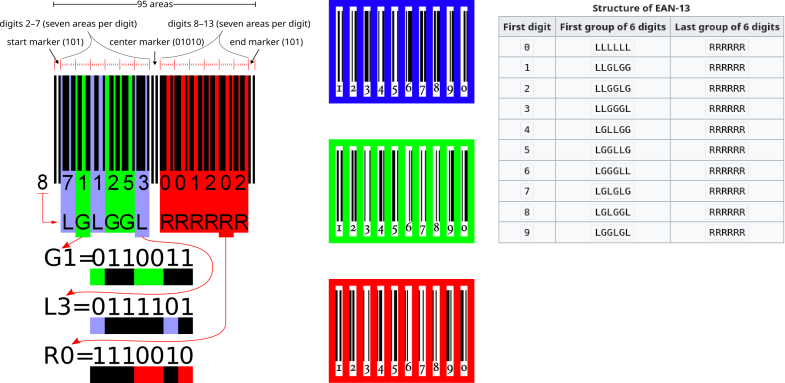
\includegraphics[keepaspectratio,width=0.9\textwidth,height=0.7\textheight]{EAN-13.png}
  \caption{EAN-13 barcode}\label{fig-EAN13}
\end{figure}

\framebreak
\begin{verbatim}
Digits:   8  7  1  1  2  5  3  0  0  1  2  0
Weights:  1  3  1  3  1  3  1  3  1  3  1  3
\end{verbatim}
\begin{eqnarray}
  (8 \cdot 1)+(7 \cdot 3)+(1 \cdot 1)+(1 \cdot 3)+(2 \cdot 1)+(5 \cdot 3)+(3 \cdot 1)+&\nonumber\\
  (0 \cdot 3)+(0 \cdot 1)+(1 \cdot 3)+(2 \cdot 1) + (0 \cdot 3) &=&\nonumber\\
  8+21+1+3+2+15+3+0+0+3+2+0 &=& 58
\end{eqnarray}
\begin{eqnarray}
  (58+x) &\equiv& 0 \mod 10 \nonumber\\
  x &\equiv& -58 \mod 10 \nonumber\\
  x &\equiv& 2 \mod 10
\end{eqnarray}

Os códigos L possuem paridade ímpar enquanto os códigos G e R possuem paridade par.
Além disso os códigos L e G começam com 0 e os códigos R começam com 1.
Desta forma, o código de barras pode ser escaneado em qualquer direção e o software
é capaz de detectar qual é a direção correta do código.


\end{frame}


\end{document}

